\documentclass[8pt,t,usepdftitle=false]{beamer}
\usetheme{Juelich}
\usepackage{setspace}
\usepackage[official]{eurosym}
\usepackage{bm}
\usepackage{mathtools}
%\usepackage{enumitem}\setitemize{itemsep=1ex}
\usepackage[%
backend=bibtex,
style=authoryear,
doi=true,
isbn=true,
url=true,
eprint=false,
sorting=nyt]{biblatex}
\addbibresource{refs.bib}
\usepackage{listings}
\lstset{
    basicstyle=\footnotesize,
    commentstyle=\color{blue},
    stringstyle=\sffamily,
    texcl=false,
    numbers=left,
    numberstyle=\tiny,
    stepnumber=1,
    numbersep=2ex,
    showstringspaces=false,
    captionpos=b,
    lineskip=0ex,%1pt,
    aboveskip=10pt,
    belowskip=10pt,
    frame=tb,
    showlines=true
}

\fzjset{
  title=regular,
  subtitle=regular,
  part=regular,
}

\setbeamerfont{title}{size*={10pt}{10pt},series=\bfseries}
\setbeamerfont{subtitle}{size*={12pt}{12pt},series=\bfseries\color{white}}
\setbeamerfont{frametitle}{size*={14pt}{14pt},series=\bfseries}
\setbeamertemplate{navigation symbols}{}

\setbeamertemplate{itemize/enumerate body begin}{\normalsize}
\setbeamertemplate{itemize/enumerate subbody begin}{\normalsize}
\setbeamertemplate{itemize/enumerate subsubbody begin}{\normalsize}
\setbeamertemplate{itemize/enumerate subsubsubbody begin}{\normalsize}

\mode<presentation>
{
  \usetheme{default}
  %% \setbeamercovered{transparent}
  \usefonttheme{professionalfonts}
  \usefonttheme{structurebold}
  \usecolortheme[rgb={0,0.3,0.6}]{structure}
}

% Delete this, if you do not want the table of contents to pop up at
% the beginning of each subsection:
% \AtBeginSection[]
% {
%   %\begin{frame}<beamer>
%     \begin{frame}[plain]
%     \frametitle{Outline}
%     \tableofcontents[currentsection]
%   \end{frame}
% }

\setlength{\leftmarginii}{3ex}

\setbeamercolor{alerted text}{fg=fzjblue}

\renewcommand{\arraystretch}{1.5}

\hypersetup{colorlinks,linkcolor=fzjblue,urlcolor=fzjblue,citecolor=fzjblue}

%%%%%%%%%%%%%%%%%%%%%%%%%%%%%%%%%%%%%%%%%%%%%%%%%%%%%%%%%%%%%%%%%%%%%%%%%%%%%%%%%%%%%%%%%%%%%%%%%
%% macros
\def\figpath{./figures}

\hypersetup{
  pdftitle={EITN fall school: proposal of student's project},
  pdfauthor={Tom Tetzlaff}
  }

%%%%%%%%%%%%%%%%%%%%%%%%%%%%%%%%%%%%%%%%%%%%%%%%%%%%%%%%%%%%%%%%%%%%%%%%%%%%%%%%%%
\title{%
  {\normalsize\normalfont project proposal:}\\[1ex]
  {\large\bf Effect of homeostatic regulation on dynamics of recurrent neuronal networks}\\[1ex]
}
\subtitle{%
  {\normalsize\mdseries Tom Tetzlaff}%
  %{\hfill\tiny\url{t.tetzlaff{at}fz-juelich.de}}\\
  {\hfill\tiny\texttt{t.tetzlaff@fz-juelich.de}}\\  
  {\footnotesize\mdseries Institute of Neuroscience and Medicine (INM-6), J\"ulich Research Centre and JARA}
  %{\hfill\tiny\url{http://www.csn.fz-juelich.de}}
  {\hfill\tiny\texttt{http://www.csn.fz-juelich.de}}
  \\
  {\tiny\mdseries EITN fall school, Paris, 20.09.2023}
  {\hfill\tiny\texttt{https://github.com/tomtetzlaff/2023\_eitnfallschool}}  
}
\date{}
\author{}
\institute{}

%%%%%%%%%%%%%%%%%%%%%%%%%%%%%%%%%%%%%%%%%%%%%%%%%%%%%%%%%%%%%%%%%%%%%%%%%%%%%%%%%%%%%%%%%%%%%%%%%
\begin{document}
\maketitle

%%%%%%%%%%%%%%%%%%%%%%%%%%%%%%%%%%%%%%%%%%%%%%%%%%%%%%%%%%%%%%%%%%%%%%%%%%%%%%%%%%%%%%%%%%%%%%%%%
\begin{frame}[plain]
  \begin{center}
    \parbox{0.9\linewidth}{
      \vspace{0.95\textheight}
      \parbox[c]{0.1\linewidth}{%
        \href{https://creativecommons.org/licenses/by-sa/4.0}{%
          
\includegraphics[width=\linewidth]{\figpath/by-sa.png}}}
      \parbox[c]{0.9\linewidth}{\scriptsize%
        ~~{}This presentation is provided under the terms of the Creative Commons Attribution-ShareAlike License 4.0.
      }
    }    
  \end{center}
\end{frame}
%%%%%%%%%%%%%%%%%%%%%%%%%%%%%%%%%%%%%%%%%%%%%%%%%%%%%%%%%%%%%%%%%%%%%%%%%%%%%%%%%%%%%%%%%%%%%%%%%
\def\ttl{Outline}
\pdfbookmark[2]{Outline}{Outline}
\begin{frame}[plain]
  \frametitle{\ttl}
  \tableofcontents
\end{frame}
%%%%%%%%%%%%%%%%%%%%%%%%%%%%%%%%%%%%%%%%%%%%%%%%%%%%%%%%%%%%%%%%%%%%%%%%%%%%%%%%%%%%%%%%%%%%%%%%%
\def\ttl{Background}\section{\ttl}
\begin{frame}[t,plain]
  \frametitle{\ttl}
  \begin{itemize}\itemsep1ex
  \item<1-> both in nature and in Computational Neuroscience, neuronal network dynamics can become unstable, leading either
    \begin{itemize}\itemsep1ex
    \item to an explosion of network activity or other pathological states, or
    \item to dying out of network activity
    \end{itemize}
    often accompanied by a loss of network functionality
  \item<2-> typical causes:
    \begin{itemize}\itemsep1ex
    \item<2-> strong excitatory feedback:
      \begin{itemize}\itemsep1ex
      \item[] firing activity $\uparrow$
      \item[$\curvearrowright$]
        synaptic input $\uparrow$
      \item[$\curvearrowright$]
        firing activity $\uparrow$
      \item[\ldots]
      \end{itemize}
    \item<3-> correlation-based plasticity dynamics, such as spike-timing-dependent plasticity (STDP):
      \begin{itemize}\itemsep1ex
      \item[] correlations in firing activity of a pair neurons $\uparrow$
      \item[$\curvearrowright$] synaptic coupling between them $\uparrow$
      \item[$\curvearrowright$] correlations in firing activity  $\uparrow$
      \item[\ldots]
      \end{itemize}
    \end{itemize}
  \item<4-> typical countermeasures
    \begin{itemize}\itemsep1ex
    \item Computational Neuroscience: laborious parameter tuning and/or unrealistic assumptions
    \item (healthy) brains: \emph{homeostatic regulation}
    \end{itemize}
  \end{itemize}
\end{frame}
%%%%%%%%%%%%%%%%%%%%%%%%%%%%
\begin{frame}[t,plain]
  \frametitle{\ttl}
  \framesubtitle{Known forms of homeostasis in biological neuronal networks}
  \begin{columns}
    \begin{column}{0.7\linewidth}
      \vspace*{-2ex}
      \begin{itemize}\itemsep1.5ex
      \item<1-> intrinsic plasticity \alert{(hours--days)}:
        regulation of cell-intrinsic excitability (e.g., thresholds; ``slow adaptation'') {\tiny \parencite{Naude12_e1002349}}
      \item<2-> short-term plasticity \alert{(10-1000ms)}:
        (transient) regulation of postsynaptic response amplitude (``synaptic weight'') based on presynaptic activity level
        {\tiny\parencite{Tsodyks97}}
      \item<3-> inhibitory plasticity \alert{(minutes--hours)}:
        regulation of strength of inhibitory connections controlled by pre- and postsynaptic activity (spike-timing-dependent plasticity)\\
        {\tiny \parencite{Hennequin17_557}}
      \item<4-> synaptic scaling \alert{(days)}:
        regulation of synaptic weights based on postsynaptic activity level\\
        {\tiny\parencite{Abbott00_1178,Tetzlaff11_47}}
      \item<5-> synaptic normalization \alert{(hours--days)}:
        long-term synaptic plasticity under the constraint that the total amount of synaptic ressources per neuron (e.g.~postsynaptic receptors) is constant
        {\tiny\parencite{Hartmann15_e1004640}}
      \item<6-> structural plasticity \alert{(hours-days)}:
        removal or formation of connections controlled by postsynaptic activity level (``synaptic turnover'')
        {\tiny \parencite{Butz13_e1003259,Gallinaro18_3,Gallinaro22_e1009836}}
      \item<7-> \ldots and certainly many more
      \end{itemize}      
    \end{column}
    \begin{column}{0.3\linewidth}
      %%%
      \vspace*{-0.5cm}
      \onslide<1->{
        \parbox{\linewidth}{
          {\footnotesize Intrinsic plasticity}
          \begin{center}
            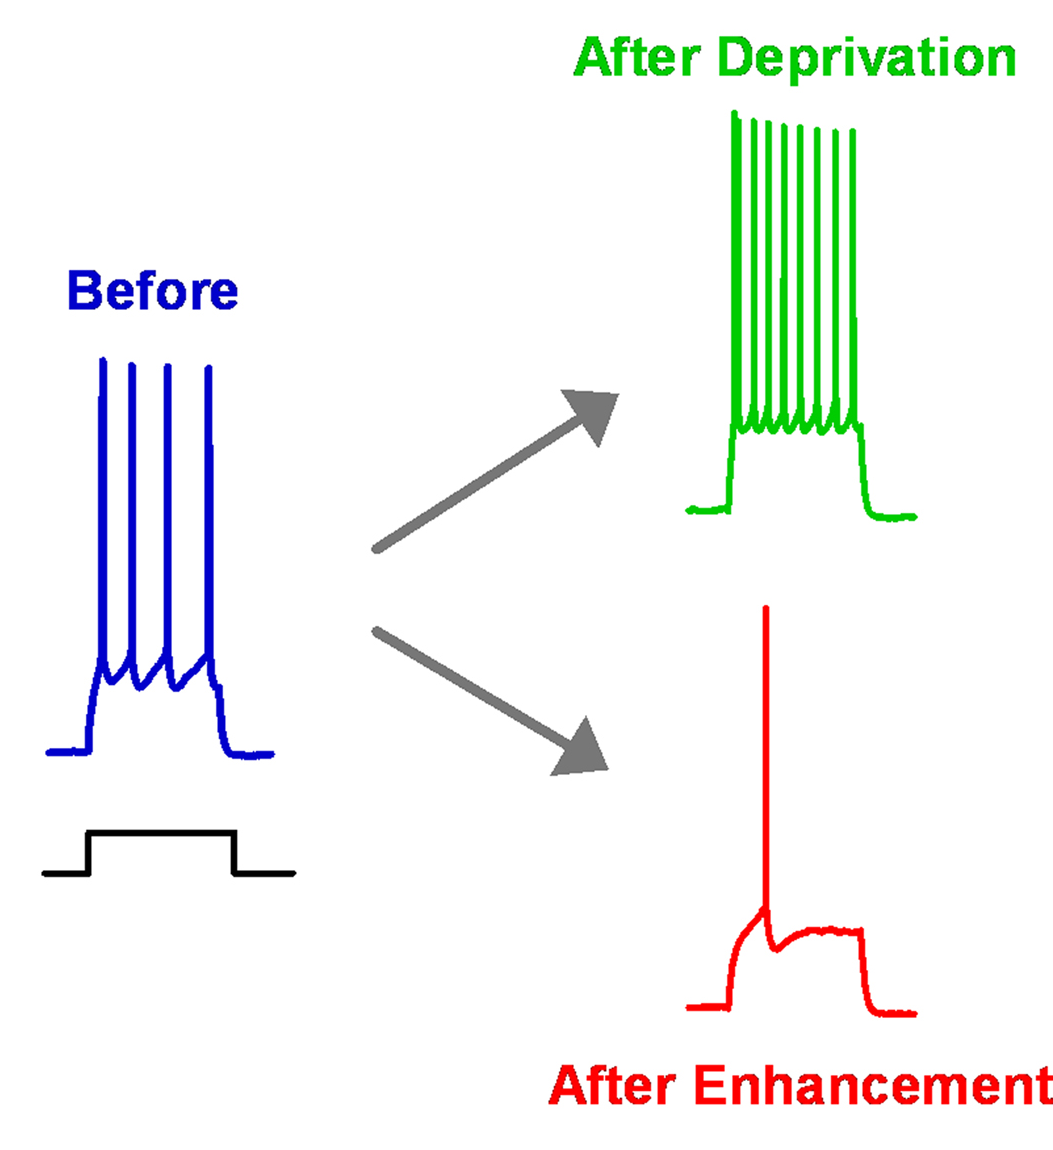
\includegraphics[width=0.4\linewidth]{figures/watt10.png}\\
            {\hspace*{\fill}\tiny \parencite{Watt10_1486}}
          \end{center}
        }}
      %%% 
      \onslide<2->{
        \parbox{\linewidth}{
          {\footnotesize Short-term plasticity}
          \begin{center}
            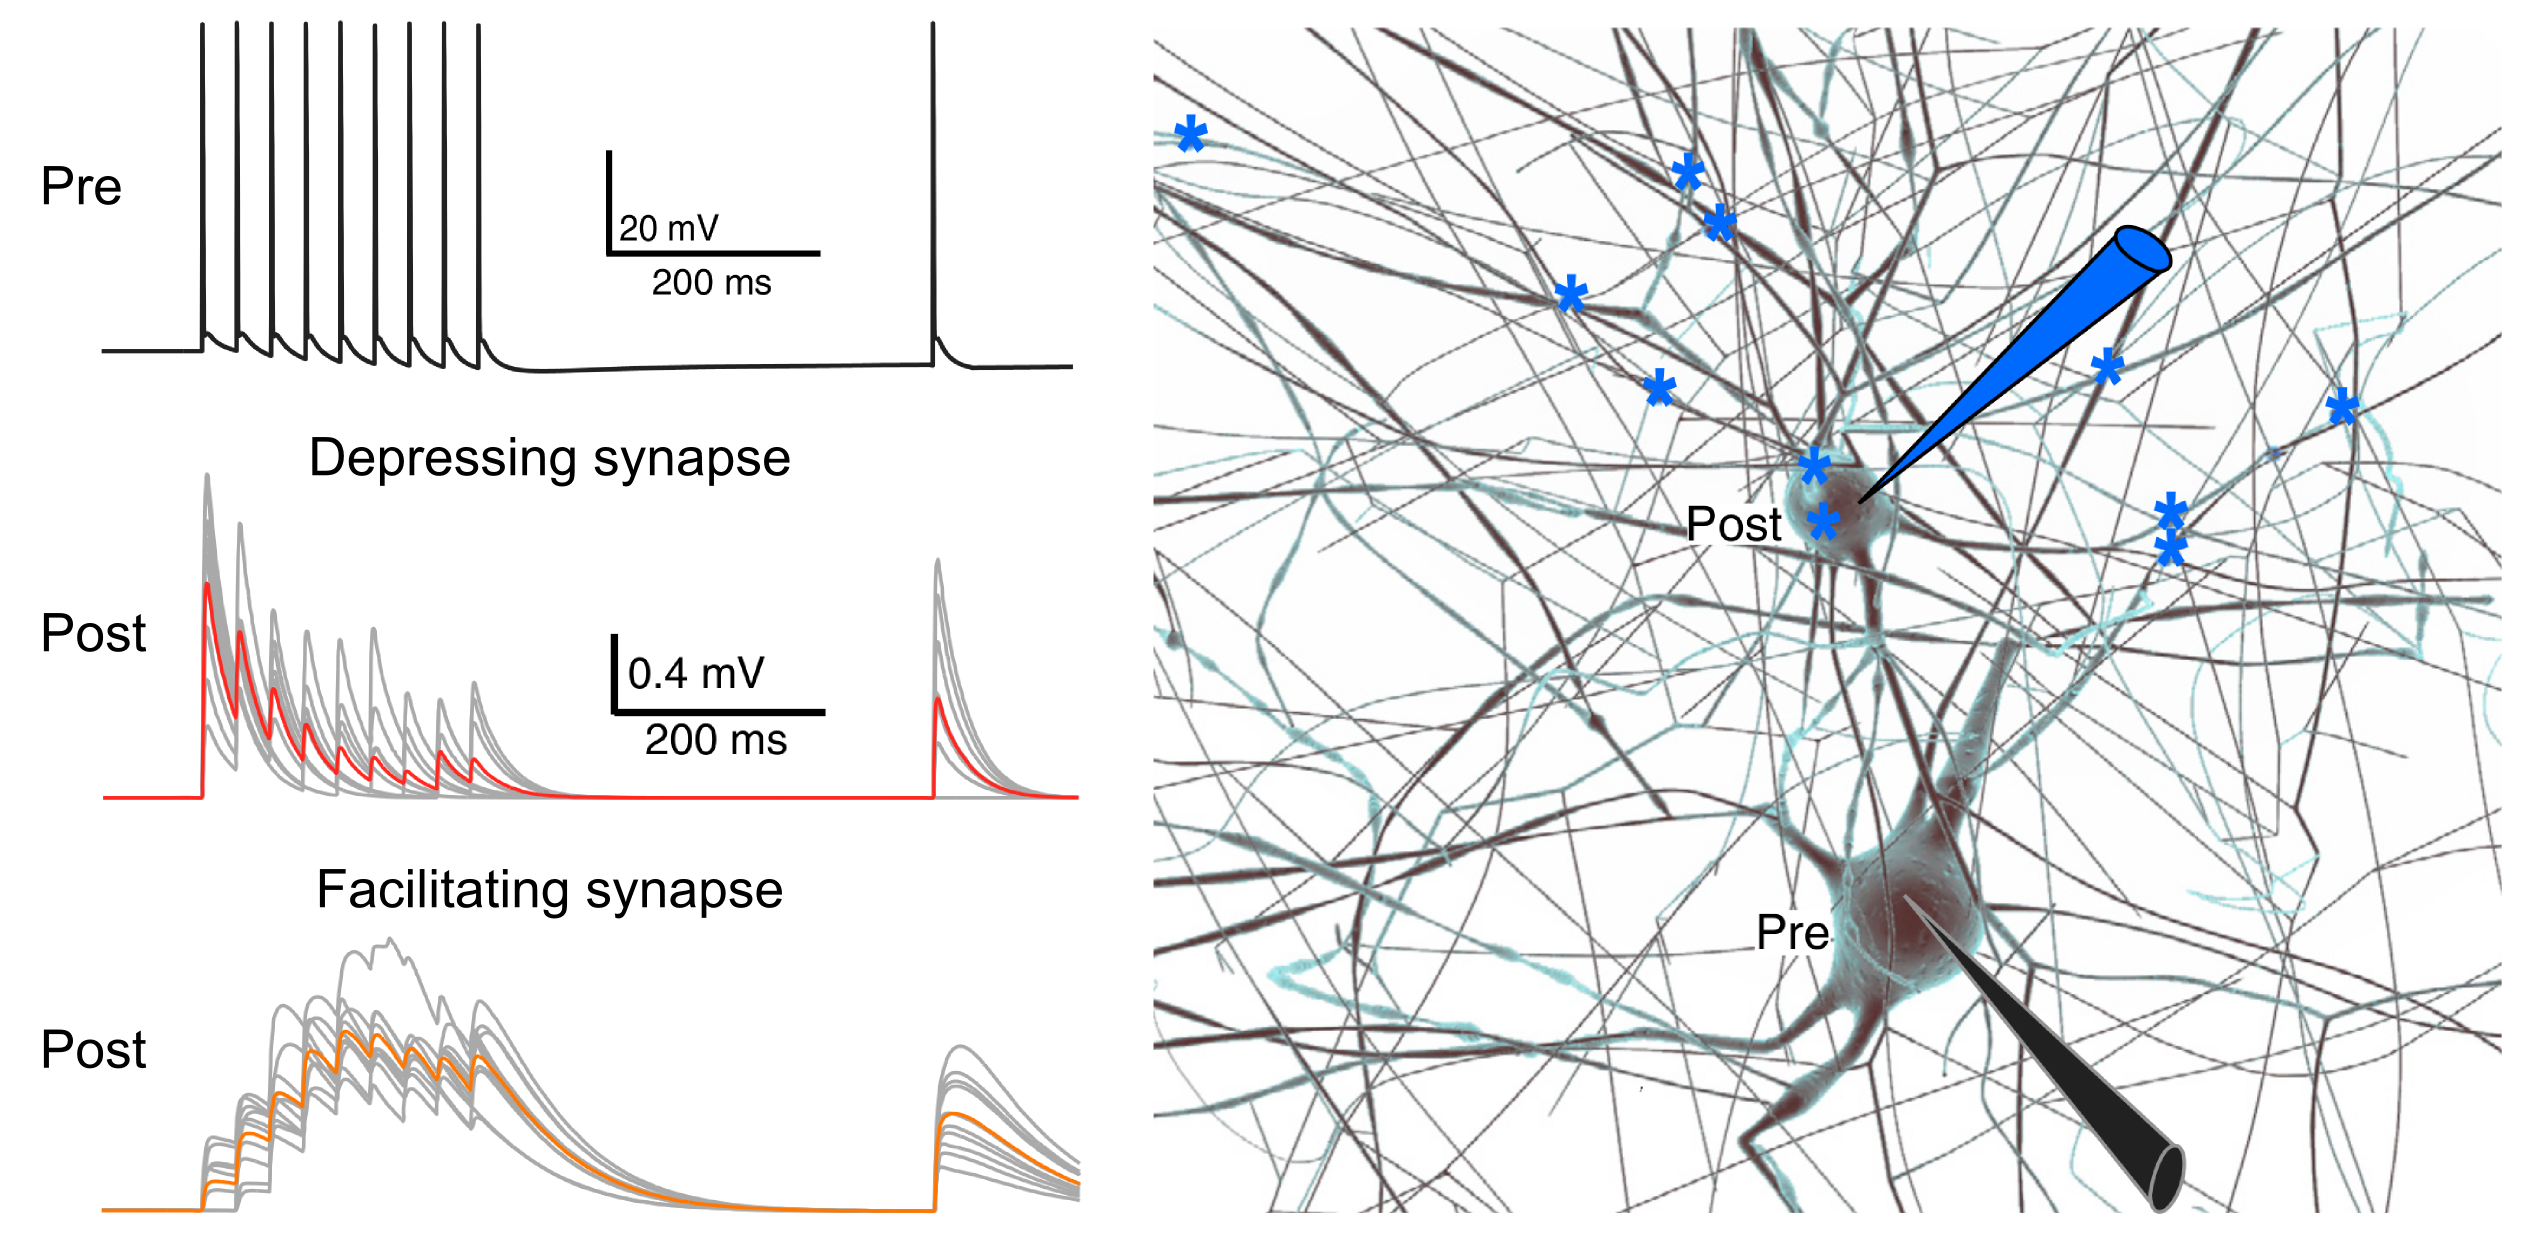
\includegraphics[width=\linewidth]{figures/markram15.png}\\
            {\hspace*{\fill}\tiny \parencite{Markram2015_456}}
          \end{center}
      }}
    %%%
    \onslide<6->{
       \parbox{\linewidth}{
        {\footnotesize Structural plasticity}
        \begin{center}
          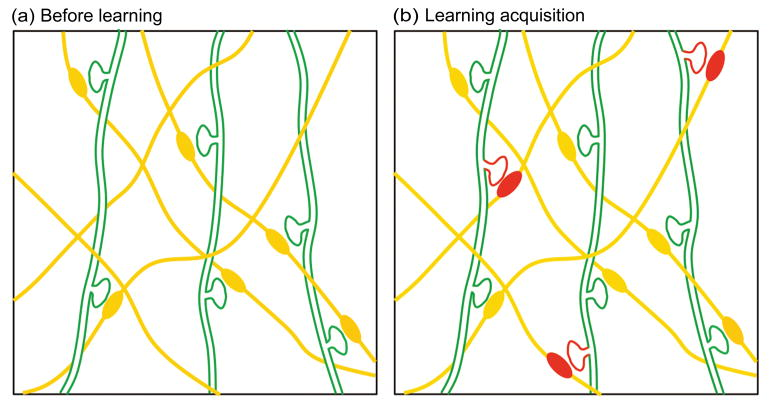
\includegraphics[width=\linewidth]{figures/fu11.png}\\
          {\hspace*{\fill}\tiny \parencite{Fu11_177}}
        \end{center}
      }}
      %%% 
    \end{column}
  \end{columns}
\end{frame}
%%%%%%%%%%%%%%%%%%%%%%%%%%%%%%%%%%%%%%%%%%%%%%%%%%%%%%%%%%%%%%%%%%%%%%%%%%%%%%%%%%%%%%%%%%%%%%%%%
\def\ttl{Questions and hypotheses}\section{\ttl}
\begin{frame}[t,plain]
  \frametitle{\ttl}
  \begin{enumerate}\itemsep2ex
  \item[1)]<1-> What biologically plausible mechanisms can effectively stabilize healthy recurrent network dynamics (low rates, asynchronous firing)?
  \item[2)]<2-> How does the presence of such mechanisms alter network dynamics, such as the dynamics in response to perturbations?
  \end{enumerate}
\end{frame}
%%%%%%%%%%%%%%%%%%%%%%%%%%%%%%%%%%%%%%%%%%%%%%%%%%%%%%%%%%%%%%%%%%%%%%%%%%%%%%%%%%%%%%%%%%%%%%%%%
\def\ttl{Proposed work plan}\section{\ttl}
\begin{frame}[t,plain]
  \frametitle{\ttl}
  \begin{columns}
    \begin{column}{0.6\linewidth}
      \begin{enumerate}\itemsep1ex
      \item<1-> implement a simple recurrent neuronal network model as presented during the NEST tutorial\\
        {\tiny (see NEST example: \texttt{balanced\_random\_network.py})}
      \item<2-> equip the model with a classical form of spike-timing-dependent plasticity in the connections between excitatory neurons\\[1ex]
        \parbox{\linewidth}{\tiny{}
          (such as proposed by \textcite{Morrison07_1437};\\
          ~see NEST synapse model \texttt{stdp\_pl\_synapse*})
        }
      \item<3-> observe how the network activity evolves into an epileptic high-activity state for high levels of synaptic potentiation (learning rate)
      \item<4-> extend the model with one (or several) of the mentioned forms of homeostasis
      \item<5-> investigate if the destabilization of network activity by strong synaptic potentiation can be prevented by the implemented form of homeostasis
      \item<6-> investigate how the implemented form of homeostasis affects network dynamics in the absence or presence of external perturbations (such as average firing rates, level of correlations in firing activity, power spectra of population activity, sensitivity to perturbations)\\
        \hspace*{\fill}{\tiny\parencite{Bachmann20_e1007790}}
      \end{enumerate}      
    \end{column}
    \begin{column}{0.4\linewidth}
      \vspace*{-7ex}
      \begin{center}
        \onslide<1->{
          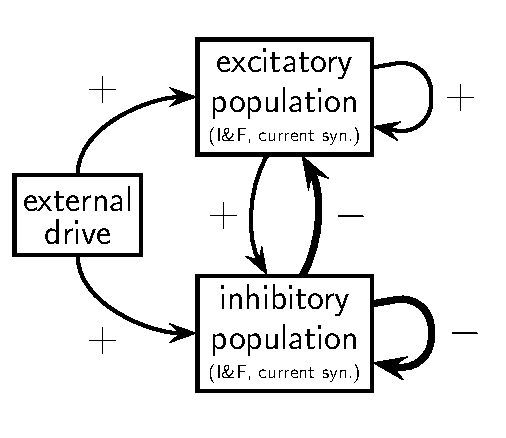
\includegraphics[width=0.7\linewidth]{figures/brunel}\\[1ex]
        }
        \onslide<2->{
          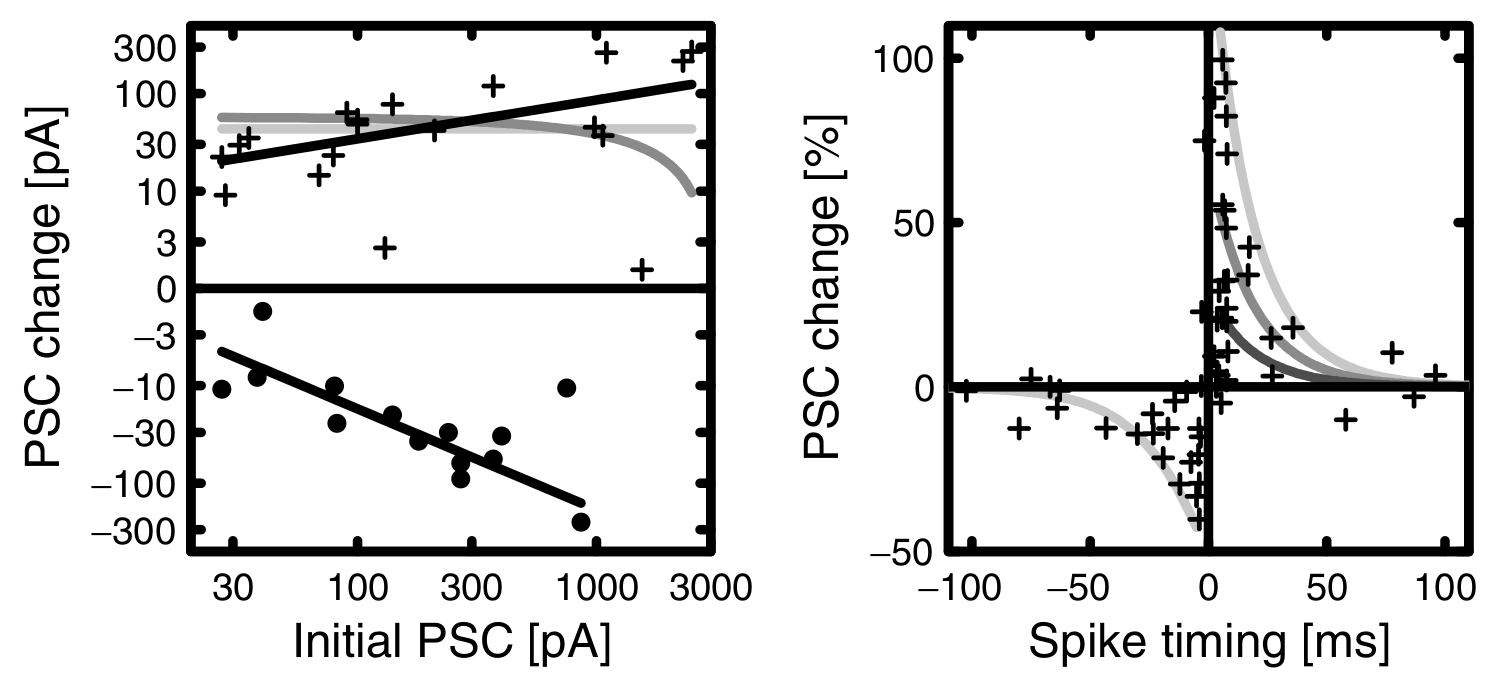
\includegraphics[width=\linewidth]{figures/Morrison07_1437_fig1.png}\\
          \hspace*{\fill}{\tiny\parencite{Morrison07_1437}}\\[1ex]
        }
        \onslide<3->{
          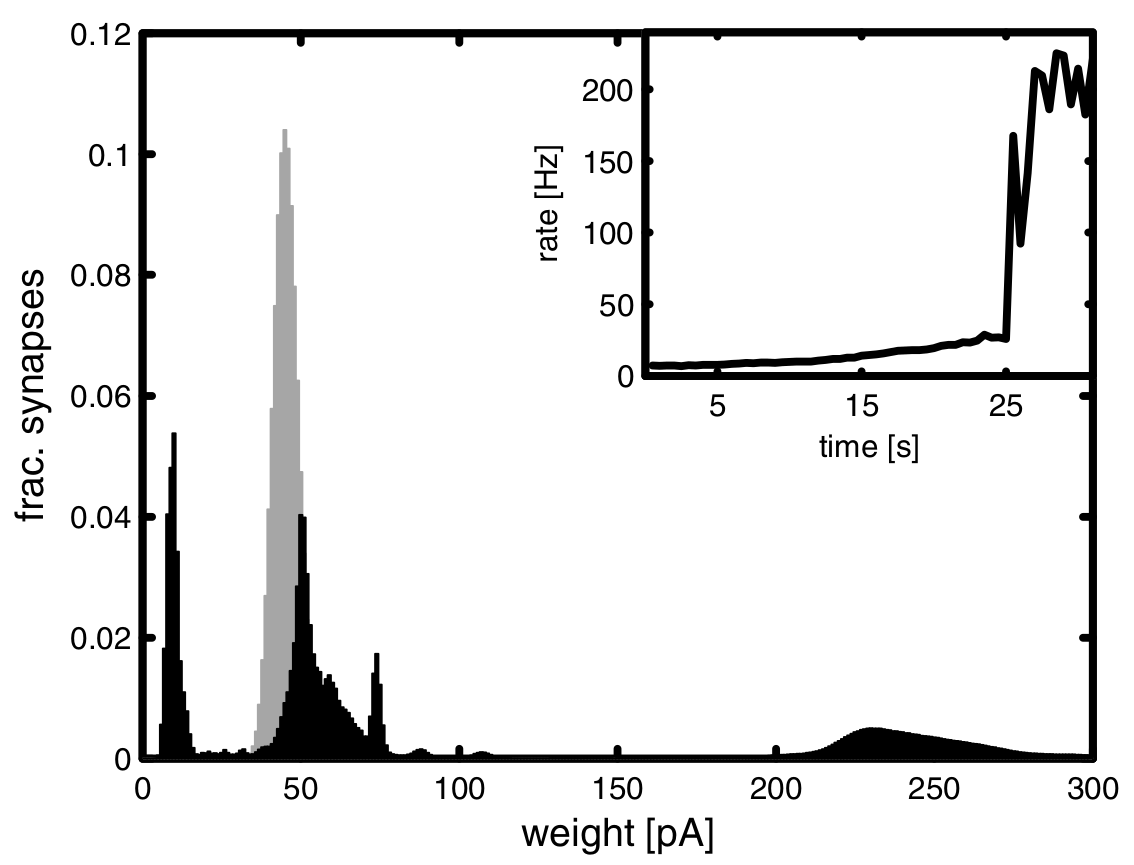
\includegraphics[width=0.8\linewidth]{figures/Morrison07_1437_fig7.png}\\
          \hspace*{\fill}{\tiny\parencite{Morrison07_1437}}\\[1ex]
        }
        \end{center}      
    \end{column}
  \end{columns}
\end{frame}
%%%%%%%%%%%%%%%%%%%%%%%%%%%%%%%%%%%%%%%%%%%%%%%%%%%%%%%%%%%%%%%%%%%%%%%%%%%%%%%%%%%%%%%%%%%%%%%%%
\begin{frame}[t,plain,allowframebreaks]
  \begin{center}
    \vspace*{\fill}
    \LARGE\emph{\it Thanks}
    \vspace*{\fill}
  \end{center}
\end{frame}
%%%%%%%%%%%%%%%%%%%%%%%%%%%%%%%%%%%%%%%%%%%%%%%%%%%%%%%%%%%%%%%%%%%%%%%%%%%%%%%%%%%%%%%%%%%%%%%%%
%% references
\setbeamertemplate{bibliography item}{}  %% remove document icon
\def\ttl{References}\section*{\ttl}
\begin{frame}[t,plain,allowframebreaks]  
  \frametitle{\ttl}
  \bibitemsep1ex
  \renewcommand{\bibfont}{\normalfont\small}
  \printbibliography
\end{frame}
%%%%%%%%%%%%%%%%%%%%%%%%%%%%%%%%%%%%%%%%%%%%%%%%%%%%%%%%%%%%%%%%%%%%%%%%%%%%%%%%%%%%%%%%%%%%%%%%%
\end{document}
%%%%%%%%%%%%%%%%%%%%%%%%%%%%%%%%%%%%%%%%%%%%%%%%%%%%%%%%%%%%%%%%%%%%%%%%%%%%%%%%%%%%%%%%%%%%%%%%%
%%%%%%%%%%%%%%%%%%%%%%%%%%%%%%%%%%%%%%%%%%%%%%%%%%%%%%%%%%%%%%%%%%%%%%%%%%%%%%%%%%%%%%%%%%%%%%%%%

%%% Local Variables:
%%% mode: latex
%%% TeX-master: t
%%% End:

notes:

Effenberger F, Jost J, Levina A (2015) Self-organization in Balanced State Networks by STDP and Homeostatic Plasticity. PLoS Comput Biol 11(9): e1004420. https://doi.org/10.1371/journal.pcbi.1004420
https://journals.plos.org/ploscompbiol/article?id=10.1371/journal.pcbi.1004420

